\begin{figure}[htbp]
\centering
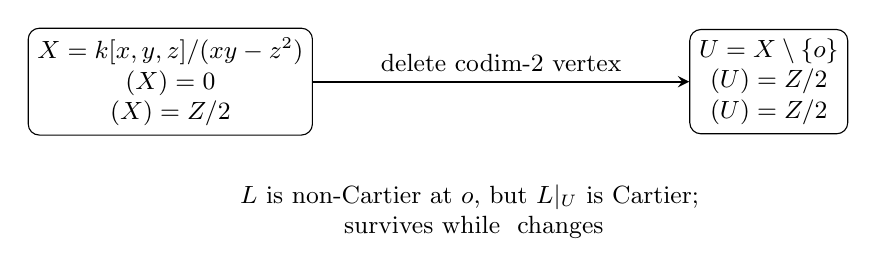
\begin{tikzpicture}[>=stealth,every node/.style={font=\small}]
\node[draw,rounded corners,align=center] (x) at (-3.8,0) {$X=\Spec k[x,y,z]/(xy-z^2)$\\$\Pic(X)=0$\\$\Cl(X)=\mathbb Z/2$};
\node[draw,rounded corners,align=center] (u) at (3.8,0) {$U=X\setminus\{o\}$\\$\Pic(U)=\mathbb Z/2$\\$\Cl(U)=\mathbb Z/2$};
\draw[->,thick] (x)--node[above] {delete codim-$2$ vertex} (u);
\node[align=center] at (0,-1.65) {$L$ is non-Cartier at $o$, but $L|_U$ is Cartier;\\$\Cl$ survives while $\Pic$ changes};
\end{tikzpicture}
\caption{The quadric cone separates Weil divisor classes from line bundles and shows the sensitivity of Cartierness to a codimension-two singular point.}
\label{fig:vi42-cone-comparison}
\end{figure}
